
Each arm of the HRS has a pair of Vertical Drift Chambers(VDCs) to determine the particle trajectory at the focal plane. The algorithm to reconstruct the  trajectory is that the VDCs measure the drift time from the fire point to the sense wires directly and then a perpendicular distance can be calculated from the drift time. From those distances, the positron of the fire point can be determined by a linear fit. The straight line fitting from the fire points can be treated as the particle track.
Timing information is recorded by common-stop mode Time-to-Digital Converters(TDCs) and a typical TDC spectrum of a wire plane is shown in the Fig \ref{vdc_p1} and three different regions are labelled in this spectrum
\begin{figure}
 	\begin{center}
 		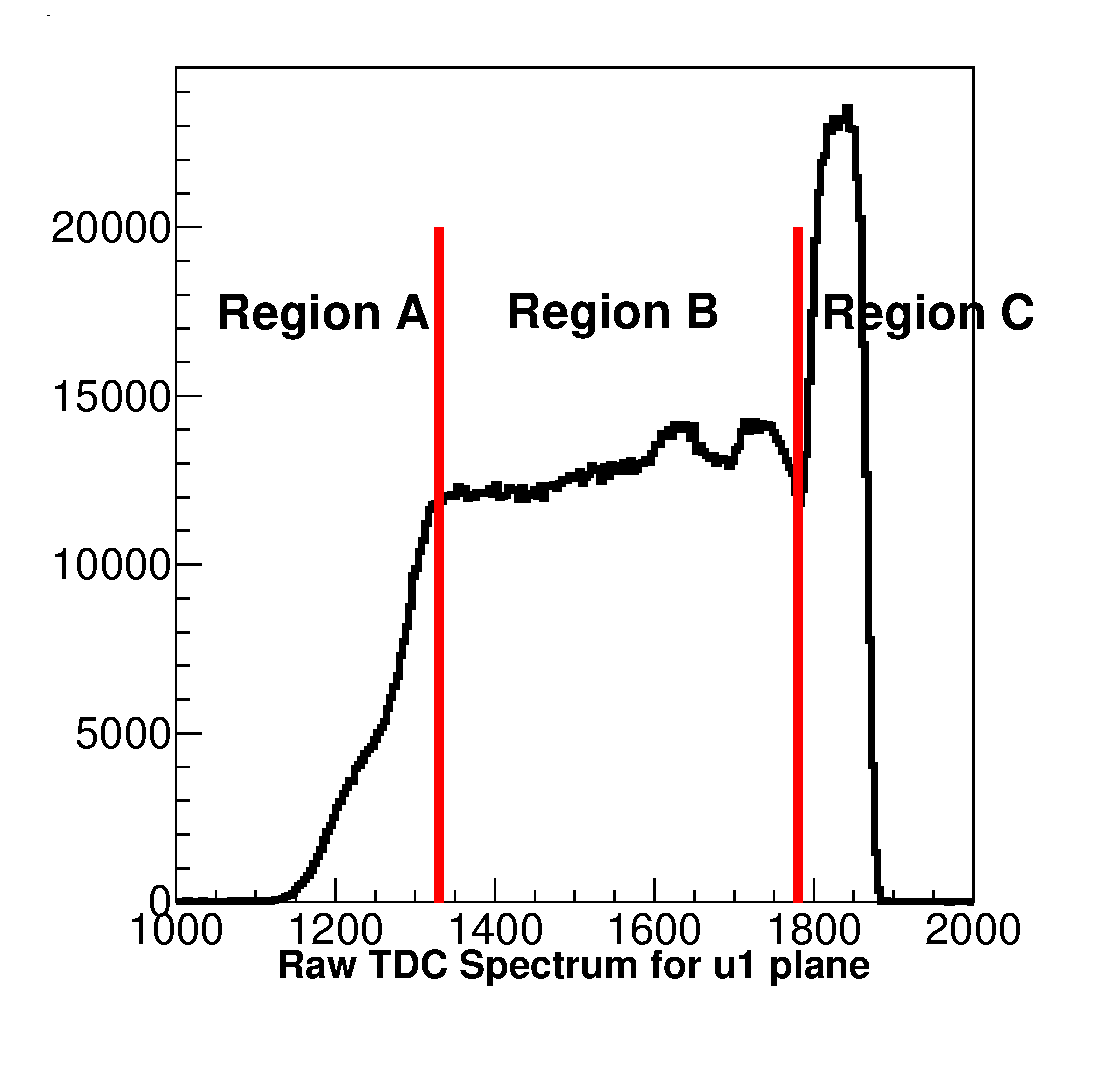
\includegraphics[width=0.4\textwidth] {./vdc_plot/vdc_cali3.eps}
 		\caption{ Raw TDC spectrum for u1 wire plane} \label{vdc_p1}
 	\end{center}
\end{figure}   
\begin{enumerate}
\item Region A: In this region, the fire point is relatively far from the sense fire and the  probability to detect a particle is low 
\item Region B: The events in these area correspond to the area in the wire plane with a uniform electric field, so the probability to detect a particle is uniform
\item Region C: The fire position for these events are very close to the sense wire and the electric field from this area is going to change to radial shape and the probability to detect a particle is going to increase in this area and since the distance from the fire point to the sense wire has a minimum limit so the right side of this area has a sharp slope. 
\end{enumerate}
Since different wire connect to the different TDC Channel and each individual TDC channel has different time offset, the VDC calibration goal is to find out the timing offset for every TDC Channel  and align the timing information in the same way. Usually the reference time is chosen at the sharp slope position of Region C($t_{0}$) as shown in Fig \ref{vdc_p1} and Fig \ref{vdc_p2} shows the offset corrected time at four wire planes after calibration. 
\begin{figure}
 	\begin{center}
 		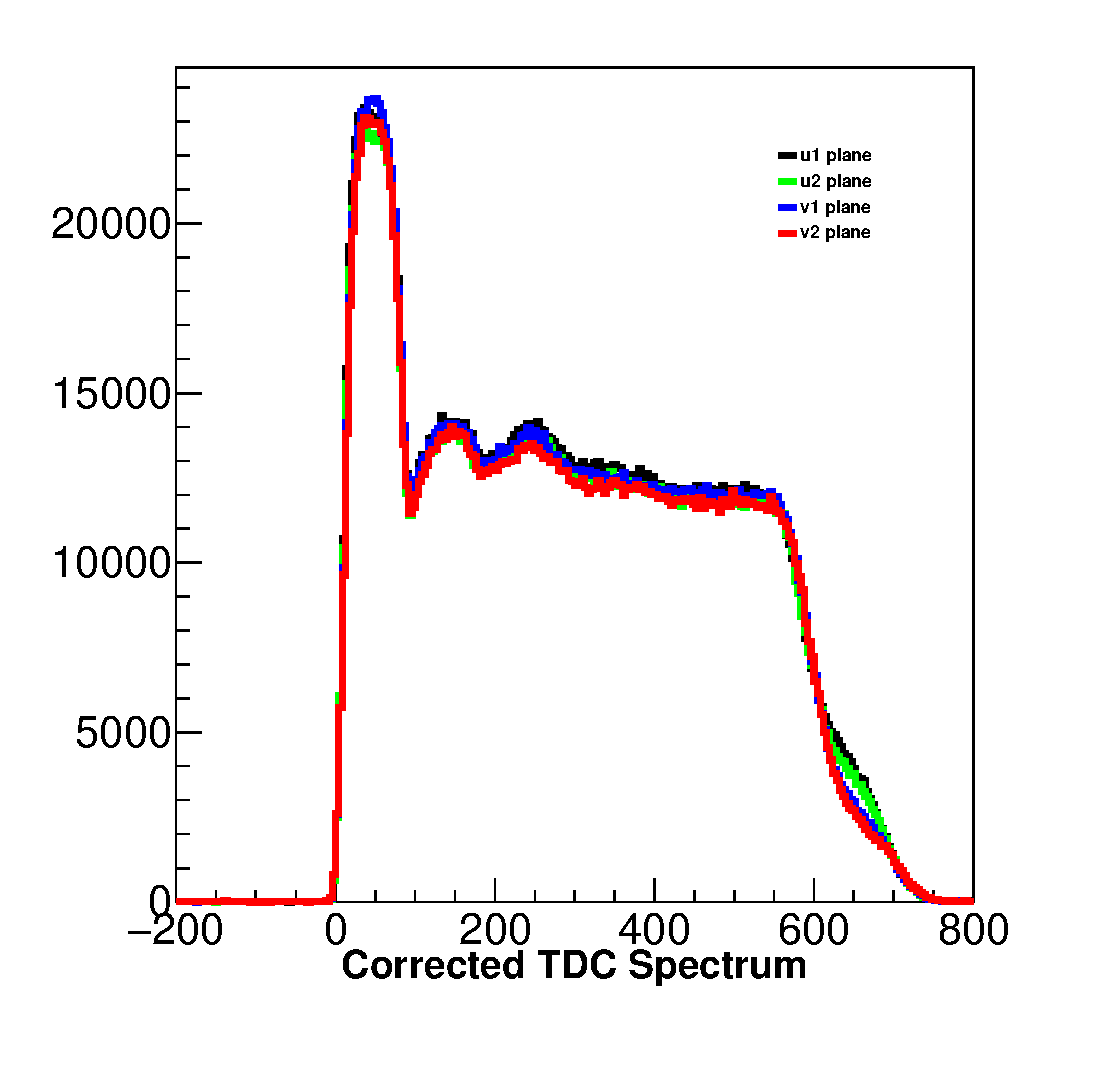
\includegraphics[width=0.4\textwidth] {./vdc_plot/vdc_cali2.eps}
 		\caption{ Corrected TDC spectrum for the 4 wire plane after calibration } \label{vdc_p2}
 	\end{center}
\end{figure}   
